\section{Introduction to State-Space Model}
\label{state:sec:ssm}
Reference: \href{http://apmonitor.com/pdc/index.php/Main/StateSpaceModel}{State-Space Models}.

The state of a dynamic system is a set of physical quantities, the specification of which completely determines the evolution of the system. The state variables are minimum set of variables that fully describe (enough information) the system. 

Many dynamic systems can be represented by using differential equations, since how the systems are changing is actually a function of current state. 
%For instance, if we want to depict a region, where its direction of wind varies by temperature and humidity. Then, we can set them as state variables. 
% \begin{figure}[h]
% 	\centering
% 	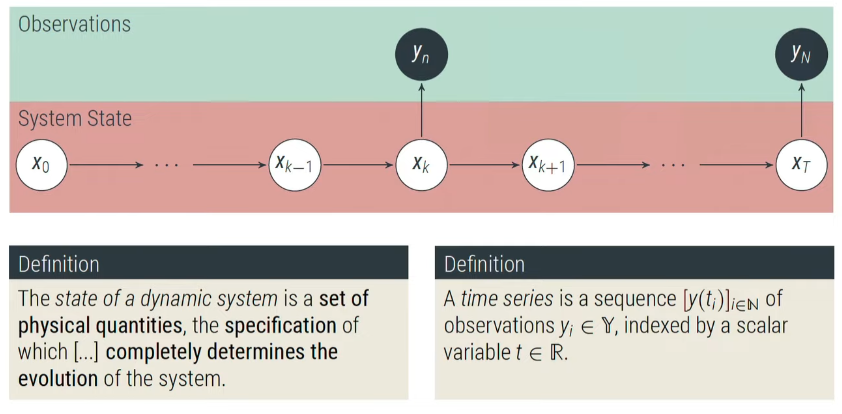
\includegraphics[scale=0.6]{./images/state_space/state_time_series.png}
% \end{figure}
% A probabilistic state-space model is a Bayesian model that defines
% \begin{itemize}
% 	\item An initial distribution $\rvx_0\sim p(\rvx_0)$ as a prior over the very first state, and for the state $\rvx_k\in \mathbb{R}^D$ and measurement $\rvy_k\in\mathbb{R}^d$ at time step $k$.
% 	\item A dynamics model as the prior over the (forward) state transitions.
% 		$$\rvx_k\sim p(\rvx_k|\rvx_{k-1}), $$
% 	\item A measurement model is a generative model for observations of the latent state.
% 		$$\rvy_k\sim p(\rvy_k|\rvx_{k}), $$
% \end{itemize}
\begin{align*}
	\dot{x} &= {A}x+{B}u,\\
	% \frac{dX}{dt} &= {A}X+{B}U,\\
	y &= {C}x+Du.
\end{align*}
The first and the second equations are known as \textit{state equation} and \textit{output equation}, respectively. The state equation tells us that how the state vector changes with the state vector and the (external) input. 

\begin{itemize}
	\item $x\in \mathbb{R}^n$: A state vector.
	\item $\dot{x}\in \mathbb{R}^n$: state derivative \ie $\big(\frac{dX}{dt}\big)$ represents the changes of the state vector. You can notice that this is a linear combination of state vector and the input vector. 
	\item $u\in \mathbb{R}^m$: Input
	\item $y\in \mathbb{R}^p$: Output
	\item $A\in \mathbb{R}^{n\times n}$: This matrix describes how the state vector influences the changes of the state vector. 
	\item $B\in \mathbb{R}^{n\times m}$: This matrix describes how the (external) input vector influences the changes of the state vector. 
	\item $C\in \mathbb{R}^{p\times n}$: Typically, an identity matrix ($I$).
	\item $D\in \mathbb{R}^{p\times m}$: Typically, zeros
\end{itemize}


\subsection{Stability}

The linear state space model is stable if all eigenvalues of $A$ are negative real numbers or have negative real parts to complex number eigenvalues. If all real parts of the eigenvalues are negative then the system is stable, meaning that any initial condition converges exponentially to a stable attracting point. If any real parts are zero then the system will not converge to a point and if the eigenvalues are positive the system is unstable and will exponentially diverge.

\subsection{First Order System in State Space}

Let's consider an example to transform a first order linear system (without time delay):
\begin{align*}
	\tau_{p}\frac{dy}{dt} &= -y+K_pu,\\
\end{align*}
where $\tau_{p}$ and $K_p$ are time constant and gain, respectively. Then, we can transform it into a state space form as follows:
\begin{align*}
	\dot{x}&= \bigg[-\frac{1}{\tau_p}\bigg]x+\bigg[\frac{K_p}{\tau_p}\bigg]u,\\
	y &= [1]x+[0]u\\
	  &= x.
\end{align*}
Here, $A=-\frac{1}{\tau_p}$, $B = \frac{K_p}{\tau_p}$, $C=1$, and $D=0$. We can solve such model by using various methods like Laplace transform. 


% If the eigenvalues of $A$ are all smaller than $0$, then the system is called \textit{stable}. 

% \begin{itemize}
% 	\item $X\in \mathbb{R}^n$ and ${dX}/{dt}$ are the state vector and the differential state vector, respectively. 
% 	\item $U$ and $Y$ are scalar input vector and scalar output vector, respectively. 
% 	\item $A$ is the system matrix.
% 	\item $B$ and $C$ are the input and the output matrices.
% 	\item $D$ is the feed-forward matrix.
% \end{itemize}


\section{Efficiently Modeling Long Sequences with Structured State-Spaces}
\label{sec:}
The state space model (SSM) can be defined as follows:
\begin{align*}
	x'(t) &= \mathbf{A}x(t)+\mathbf{B}u(t),\\
	y(t) &= \mathbf{C}x(t)+\mathbf{D}u(t).
\end{align*}

It maps a single dimensional input signal $u(t)$ to an $N$-dim latent state $x(t)$ before projecting to a one-dim output signal $y(t)$.  

Our goal is to simply use the SSM as a black-box representation in a deep sequence model, where $\rmA, \rmB, \rmC$, and $\rmD$ are parameters learned by gradient descent. We will omit the parameter $\rmD$ for exposition (or equivalently, assume $\rmD=0$, because the term $\rmD u$ can be viewed as a skip connection and is easy to compute).

An SSM maps a input $u(t)$ to a state representation vector $x(t)$ and an output $y(t)$. For simplicity, we assume the input and output are one-dimensional, and the state representation is $N$-dimensional. The first equation defines the change in $x(t)$ over time.

% \begin{lstlisting}[language=Python]
% 	def random_SSM(rng, N):
% 		a_r, b_r, c_r = jax.random.split(rng, 3)
% 		A = jax.random.uniform(a_r, (N, N))
% 		B = jax.random.uniform(b_r, (N, 1))
% 		C = jax.random.uniform(c_r, (1, N))
%     return A, B, C
% \end{lstlisting}
